\documentclass[landscape, a4paper, parskip=half, DIV=13]{scrartcl}
\usepackage[top=1.25cm, bottom=1.0cm, left=7cm, right=7cm, marginparwidth=6.0cm, marginparsep=0pt]{geometry}
\usepackage[dvipsnames]{xcolor}
\usepackage{tikz}
\usetikzlibrary{shapes.geometric}
\usepackage{fontspec}
\setmainfont{Tex Gyre Schola}
%\setmainfont[Scale=0.95]{Century Gothic}
\usepackage{contour}
\usepackage{multicol}
\setlength{\columnsep}{1cm}
\usepackage{booktabs}
\usepackage{lipsum}
\usepackage{marginnote}
\usepackage{multirow}
\usepackage{enumitem}
\usepackage{stealthships}

%\setkomafont{section}{\setmainfont{Tex Gyre Schola}\LARGE\textbf}
\setkomafont{section}{\setmainfont[Scale=0.95]{Century Gothic}\LARGE\bfseries}

% Adjust spacing before and after section headings
\RedeclareSectionCommand[
  runin=false,
  beforeskip=1.0\baselineskip,
  afterskip=0.0\baselineskip
]{section}


\pagestyle{empty}
\begin{document}
{
%\setmainfont[Scale=2.5]{Tex Gyre Schola}
\setmainfont[Scale=2.5]{Century Gothic}
\begin{center}
\Huge \textbf{Cryptoglyph}
\end{center}
}
%\marginnote{\center\includegraphics[height=2.5cm]{elephant.png}}[-4.125cm]
%\reversemarginpar\marginnote{\center\includegraphics[height=2.5cm]{donkey.png}}[-4.125cm]

\vspace{0.0cm}
\vspace{-0.5cm}

\begin{center}
{\setmainfont{Century Gothic}
\tiny
\scalebox{2.4}{
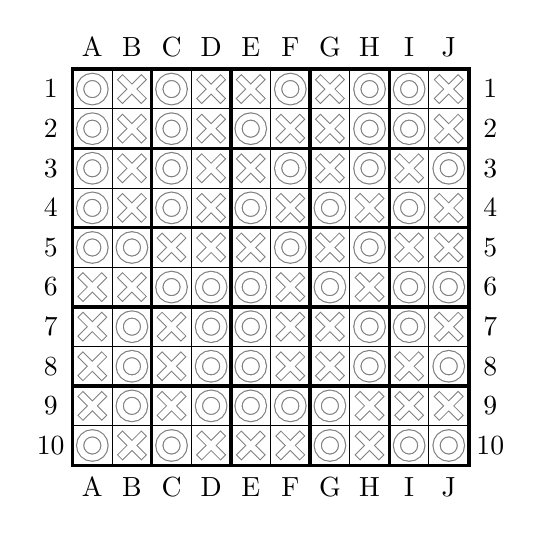
\begin{tikzpicture}
\node[draw=gray,circle,inner sep=1pt,line width=1.0416666mm] at (-0.891000in, 0.891000in) {\scriptsize\phantom{1}};
\node[draw=white,circle,inner sep=1pt,line width=0.75mm] at (-0.891000in, 0.891000in) {\scriptsize\phantom{1}};
\node[text=gray,rotate=45,inner sep=0pt] at (-0.693000in, 0.891000in) {\rule{4.3875mm}{1.0125mm}};
\node[text=gray,rotate=-45,inner sep=0pt] at (-0.693000in, 0.891000in) {\rule{4.3875mm}{1.0125mm}};
\node[text=white,rotate=45,inner sep=0pt] at (-0.693000in, 0.891000in) {\rule{4.125mm}{0.75mm}};
\node[text=white,rotate=-45,inner sep=0pt] at (-0.693000in, 0.891000in) {\rule{4.125mm}{0.75mm}};
\node[draw=gray,circle,inner sep=1pt,line width=1.0416666mm] at (-0.495000in, 0.891000in) {\scriptsize\phantom{1}};
\node[draw=white,circle,inner sep=1pt,line width=0.75mm] at (-0.495000in, 0.891000in) {\scriptsize\phantom{1}};
\node[text=gray,rotate=45,inner sep=0pt] at (-0.297000in, 0.891000in) {\rule{4.3875mm}{1.0125mm}};
\node[text=gray,rotate=-45,inner sep=0pt] at (-0.297000in, 0.891000in) {\rule{4.3875mm}{1.0125mm}};
\node[text=white,rotate=45,inner sep=0pt] at (-0.297000in, 0.891000in) {\rule{4.125mm}{0.75mm}};
\node[text=white,rotate=-45,inner sep=0pt] at (-0.297000in, 0.891000in) {\rule{4.125mm}{0.75mm}};
\node[text=gray,rotate=45,inner sep=0pt] at (-0.099000in, 0.891000in) {\rule{4.3875mm}{1.0125mm}};
\node[text=gray,rotate=-45,inner sep=0pt] at (-0.099000in, 0.891000in) {\rule{4.3875mm}{1.0125mm}};
\node[text=white,rotate=45,inner sep=0pt] at (-0.099000in, 0.891000in) {\rule{4.125mm}{0.75mm}};
\node[text=white,rotate=-45,inner sep=0pt] at (-0.099000in, 0.891000in) {\rule{4.125mm}{0.75mm}};
\node[draw=gray,circle,inner sep=1pt,line width=1.0416666mm] at (0.099000in, 0.891000in) {\scriptsize\phantom{1}};
\node[draw=white,circle,inner sep=1pt,line width=0.75mm] at (0.099000in, 0.891000in) {\scriptsize\phantom{1}};
\node[text=gray,rotate=45,inner sep=0pt] at (0.297000in, 0.891000in) {\rule{4.3875mm}{1.0125mm}};
\node[text=gray,rotate=-45,inner sep=0pt] at (0.297000in, 0.891000in) {\rule{4.3875mm}{1.0125mm}};
\node[text=white,rotate=45,inner sep=0pt] at (0.297000in, 0.891000in) {\rule{4.125mm}{0.75mm}};
\node[text=white,rotate=-45,inner sep=0pt] at (0.297000in, 0.891000in) {\rule{4.125mm}{0.75mm}};
\node[draw=gray,circle,inner sep=1pt,line width=1.0416666mm] at (0.495000in, 0.891000in) {\scriptsize\phantom{1}};
\node[draw=white,circle,inner sep=1pt,line width=0.75mm] at (0.495000in, 0.891000in) {\scriptsize\phantom{1}};
\node[draw=gray,circle,inner sep=1pt,line width=1.0416666mm] at (0.693000in, 0.891000in) {\scriptsize\phantom{1}};
\node[draw=white,circle,inner sep=1pt,line width=0.75mm] at (0.693000in, 0.891000in) {\scriptsize\phantom{1}};
\node[text=gray,rotate=45,inner sep=0pt] at (0.891000in, 0.891000in) {\rule{4.3875mm}{1.0125mm}};
\node[text=gray,rotate=-45,inner sep=0pt] at (0.891000in, 0.891000in) {\rule{4.3875mm}{1.0125mm}};
\node[text=white,rotate=45,inner sep=0pt] at (0.891000in, 0.891000in) {\rule{4.125mm}{0.75mm}};
\node[text=white,rotate=-45,inner sep=0pt] at (0.891000in, 0.891000in) {\rule{4.125mm}{0.75mm}};
\node[draw=gray,circle,inner sep=1pt,line width=1.0416666mm] at (-0.891000in, 0.693000in) {\scriptsize\phantom{1}};
\node[draw=white,circle,inner sep=1pt,line width=0.75mm] at (-0.891000in, 0.693000in) {\scriptsize\phantom{1}};
\node[text=gray,rotate=45,inner sep=0pt] at (-0.693000in, 0.693000in) {\rule{4.3875mm}{1.0125mm}};
\node[text=gray,rotate=-45,inner sep=0pt] at (-0.693000in, 0.693000in) {\rule{4.3875mm}{1.0125mm}};
\node[text=white,rotate=45,inner sep=0pt] at (-0.693000in, 0.693000in) {\rule{4.125mm}{0.75mm}};
\node[text=white,rotate=-45,inner sep=0pt] at (-0.693000in, 0.693000in) {\rule{4.125mm}{0.75mm}};
\node[draw=gray,circle,inner sep=1pt,line width=1.0416666mm] at (-0.495000in, 0.693000in) {\scriptsize\phantom{1}};
\node[draw=white,circle,inner sep=1pt,line width=0.75mm] at (-0.495000in, 0.693000in) {\scriptsize\phantom{1}};
\node[text=gray,rotate=45,inner sep=0pt] at (-0.297000in, 0.693000in) {\rule{4.3875mm}{1.0125mm}};
\node[text=gray,rotate=-45,inner sep=0pt] at (-0.297000in, 0.693000in) {\rule{4.3875mm}{1.0125mm}};
\node[text=white,rotate=45,inner sep=0pt] at (-0.297000in, 0.693000in) {\rule{4.125mm}{0.75mm}};
\node[text=white,rotate=-45,inner sep=0pt] at (-0.297000in, 0.693000in) {\rule{4.125mm}{0.75mm}};
\node[draw=gray,circle,inner sep=1pt,line width=1.0416666mm] at (-0.099000in, 0.693000in) {\scriptsize\phantom{1}};
\node[draw=white,circle,inner sep=1pt,line width=0.75mm] at (-0.099000in, 0.693000in) {\scriptsize\phantom{1}};
\node[text=gray,rotate=45,inner sep=0pt] at (0.099000in, 0.693000in) {\rule{4.3875mm}{1.0125mm}};
\node[text=gray,rotate=-45,inner sep=0pt] at (0.099000in, 0.693000in) {\rule{4.3875mm}{1.0125mm}};
\node[text=white,rotate=45,inner sep=0pt] at (0.099000in, 0.693000in) {\rule{4.125mm}{0.75mm}};
\node[text=white,rotate=-45,inner sep=0pt] at (0.099000in, 0.693000in) {\rule{4.125mm}{0.75mm}};
\node[text=gray,rotate=45,inner sep=0pt] at (0.297000in, 0.693000in) {\rule{4.3875mm}{1.0125mm}};
\node[text=gray,rotate=-45,inner sep=0pt] at (0.297000in, 0.693000in) {\rule{4.3875mm}{1.0125mm}};
\node[text=white,rotate=45,inner sep=0pt] at (0.297000in, 0.693000in) {\rule{4.125mm}{0.75mm}};
\node[text=white,rotate=-45,inner sep=0pt] at (0.297000in, 0.693000in) {\rule{4.125mm}{0.75mm}};
\node[draw=gray,circle,inner sep=1pt,line width=1.0416666mm] at (0.495000in, 0.693000in) {\scriptsize\phantom{1}};
\node[draw=white,circle,inner sep=1pt,line width=0.75mm] at (0.495000in, 0.693000in) {\scriptsize\phantom{1}};
\node[draw=gray,circle,inner sep=1pt,line width=1.0416666mm] at (0.693000in, 0.693000in) {\scriptsize\phantom{1}};
\node[draw=white,circle,inner sep=1pt,line width=0.75mm] at (0.693000in, 0.693000in) {\scriptsize\phantom{1}};
\node[text=gray,rotate=45,inner sep=0pt] at (0.891000in, 0.693000in) {\rule{4.3875mm}{1.0125mm}};
\node[text=gray,rotate=-45,inner sep=0pt] at (0.891000in, 0.693000in) {\rule{4.3875mm}{1.0125mm}};
\node[text=white,rotate=45,inner sep=0pt] at (0.891000in, 0.693000in) {\rule{4.125mm}{0.75mm}};
\node[text=white,rotate=-45,inner sep=0pt] at (0.891000in, 0.693000in) {\rule{4.125mm}{0.75mm}};
\node[draw=gray,circle,inner sep=1pt,line width=1.0416666mm] at (-0.891000in, 0.495000in) {\scriptsize\phantom{1}};
\node[draw=white,circle,inner sep=1pt,line width=0.75mm] at (-0.891000in, 0.495000in) {\scriptsize\phantom{1}};
\node[text=gray,rotate=45,inner sep=0pt] at (-0.693000in, 0.495000in) {\rule{4.3875mm}{1.0125mm}};
\node[text=gray,rotate=-45,inner sep=0pt] at (-0.693000in, 0.495000in) {\rule{4.3875mm}{1.0125mm}};
\node[text=white,rotate=45,inner sep=0pt] at (-0.693000in, 0.495000in) {\rule{4.125mm}{0.75mm}};
\node[text=white,rotate=-45,inner sep=0pt] at (-0.693000in, 0.495000in) {\rule{4.125mm}{0.75mm}};
\node[draw=gray,circle,inner sep=1pt,line width=1.0416666mm] at (-0.495000in, 0.495000in) {\scriptsize\phantom{1}};
\node[draw=white,circle,inner sep=1pt,line width=0.75mm] at (-0.495000in, 0.495000in) {\scriptsize\phantom{1}};
\node[text=gray,rotate=45,inner sep=0pt] at (-0.297000in, 0.495000in) {\rule{4.3875mm}{1.0125mm}};
\node[text=gray,rotate=-45,inner sep=0pt] at (-0.297000in, 0.495000in) {\rule{4.3875mm}{1.0125mm}};
\node[text=white,rotate=45,inner sep=0pt] at (-0.297000in, 0.495000in) {\rule{4.125mm}{0.75mm}};
\node[text=white,rotate=-45,inner sep=0pt] at (-0.297000in, 0.495000in) {\rule{4.125mm}{0.75mm}};
\node[text=gray,rotate=45,inner sep=0pt] at (-0.099000in, 0.495000in) {\rule{4.3875mm}{1.0125mm}};
\node[text=gray,rotate=-45,inner sep=0pt] at (-0.099000in, 0.495000in) {\rule{4.3875mm}{1.0125mm}};
\node[text=white,rotate=45,inner sep=0pt] at (-0.099000in, 0.495000in) {\rule{4.125mm}{0.75mm}};
\node[text=white,rotate=-45,inner sep=0pt] at (-0.099000in, 0.495000in) {\rule{4.125mm}{0.75mm}};
\node[draw=gray,circle,inner sep=1pt,line width=1.0416666mm] at (0.099000in, 0.495000in) {\scriptsize\phantom{1}};
\node[draw=white,circle,inner sep=1pt,line width=0.75mm] at (0.099000in, 0.495000in) {\scriptsize\phantom{1}};
\node[text=gray,rotate=45,inner sep=0pt] at (0.297000in, 0.495000in) {\rule{4.3875mm}{1.0125mm}};
\node[text=gray,rotate=-45,inner sep=0pt] at (0.297000in, 0.495000in) {\rule{4.3875mm}{1.0125mm}};
\node[text=white,rotate=45,inner sep=0pt] at (0.297000in, 0.495000in) {\rule{4.125mm}{0.75mm}};
\node[text=white,rotate=-45,inner sep=0pt] at (0.297000in, 0.495000in) {\rule{4.125mm}{0.75mm}};
\node[draw=gray,circle,inner sep=1pt,line width=1.0416666mm] at (0.495000in, 0.495000in) {\scriptsize\phantom{1}};
\node[draw=white,circle,inner sep=1pt,line width=0.75mm] at (0.495000in, 0.495000in) {\scriptsize\phantom{1}};
\node[text=gray,rotate=45,inner sep=0pt] at (0.693000in, 0.495000in) {\rule{4.3875mm}{1.0125mm}};
\node[text=gray,rotate=-45,inner sep=0pt] at (0.693000in, 0.495000in) {\rule{4.3875mm}{1.0125mm}};
\node[text=white,rotate=45,inner sep=0pt] at (0.693000in, 0.495000in) {\rule{4.125mm}{0.75mm}};
\node[text=white,rotate=-45,inner sep=0pt] at (0.693000in, 0.495000in) {\rule{4.125mm}{0.75mm}};
\node[draw=gray,circle,inner sep=1pt,line width=1.0416666mm] at (0.891000in, 0.495000in) {\scriptsize\phantom{1}};
\node[draw=white,circle,inner sep=1pt,line width=0.75mm] at (0.891000in, 0.495000in) {\scriptsize\phantom{1}};
\node[draw=gray,circle,inner sep=1pt,line width=1.0416666mm] at (-0.891000in, 0.297000in) {\scriptsize\phantom{1}};
\node[draw=white,circle,inner sep=1pt,line width=0.75mm] at (-0.891000in, 0.297000in) {\scriptsize\phantom{1}};
\node[text=gray,rotate=45,inner sep=0pt] at (-0.693000in, 0.297000in) {\rule{4.3875mm}{1.0125mm}};
\node[text=gray,rotate=-45,inner sep=0pt] at (-0.693000in, 0.297000in) {\rule{4.3875mm}{1.0125mm}};
\node[text=white,rotate=45,inner sep=0pt] at (-0.693000in, 0.297000in) {\rule{4.125mm}{0.75mm}};
\node[text=white,rotate=-45,inner sep=0pt] at (-0.693000in, 0.297000in) {\rule{4.125mm}{0.75mm}};
\node[draw=gray,circle,inner sep=1pt,line width=1.0416666mm] at (-0.495000in, 0.297000in) {\scriptsize\phantom{1}};
\node[draw=white,circle,inner sep=1pt,line width=0.75mm] at (-0.495000in, 0.297000in) {\scriptsize\phantom{1}};
\node[text=gray,rotate=45,inner sep=0pt] at (-0.297000in, 0.297000in) {\rule{4.3875mm}{1.0125mm}};
\node[text=gray,rotate=-45,inner sep=0pt] at (-0.297000in, 0.297000in) {\rule{4.3875mm}{1.0125mm}};
\node[text=white,rotate=45,inner sep=0pt] at (-0.297000in, 0.297000in) {\rule{4.125mm}{0.75mm}};
\node[text=white,rotate=-45,inner sep=0pt] at (-0.297000in, 0.297000in) {\rule{4.125mm}{0.75mm}};
\node[draw=gray,circle,inner sep=1pt,line width=1.0416666mm] at (-0.099000in, 0.297000in) {\scriptsize\phantom{1}};
\node[draw=white,circle,inner sep=1pt,line width=0.75mm] at (-0.099000in, 0.297000in) {\scriptsize\phantom{1}};
\node[text=gray,rotate=45,inner sep=0pt] at (0.099000in, 0.297000in) {\rule{4.3875mm}{1.0125mm}};
\node[text=gray,rotate=-45,inner sep=0pt] at (0.099000in, 0.297000in) {\rule{4.3875mm}{1.0125mm}};
\node[text=white,rotate=45,inner sep=0pt] at (0.099000in, 0.297000in) {\rule{4.125mm}{0.75mm}};
\node[text=white,rotate=-45,inner sep=0pt] at (0.099000in, 0.297000in) {\rule{4.125mm}{0.75mm}};
\node[draw=gray,circle,inner sep=1pt,line width=1.0416666mm] at (0.297000in, 0.297000in) {\scriptsize\phantom{1}};
\node[draw=white,circle,inner sep=1pt,line width=0.75mm] at (0.297000in, 0.297000in) {\scriptsize\phantom{1}};
\node[text=gray,rotate=45,inner sep=0pt] at (0.495000in, 0.297000in) {\rule{4.3875mm}{1.0125mm}};
\node[text=gray,rotate=-45,inner sep=0pt] at (0.495000in, 0.297000in) {\rule{4.3875mm}{1.0125mm}};
\node[text=white,rotate=45,inner sep=0pt] at (0.495000in, 0.297000in) {\rule{4.125mm}{0.75mm}};
\node[text=white,rotate=-45,inner sep=0pt] at (0.495000in, 0.297000in) {\rule{4.125mm}{0.75mm}};
\node[draw=gray,circle,inner sep=1pt,line width=1.0416666mm] at (0.693000in, 0.297000in) {\scriptsize\phantom{1}};
\node[draw=white,circle,inner sep=1pt,line width=0.75mm] at (0.693000in, 0.297000in) {\scriptsize\phantom{1}};
\node[text=gray,rotate=45,inner sep=0pt] at (0.891000in, 0.297000in) {\rule{4.3875mm}{1.0125mm}};
\node[text=gray,rotate=-45,inner sep=0pt] at (0.891000in, 0.297000in) {\rule{4.3875mm}{1.0125mm}};
\node[text=white,rotate=45,inner sep=0pt] at (0.891000in, 0.297000in) {\rule{4.125mm}{0.75mm}};
\node[text=white,rotate=-45,inner sep=0pt] at (0.891000in, 0.297000in) {\rule{4.125mm}{0.75mm}};
\node[draw=gray,circle,inner sep=1pt,line width=1.0416666mm] at (-0.891000in, 0.099000in) {\scriptsize\phantom{1}};
\node[draw=white,circle,inner sep=1pt,line width=0.75mm] at (-0.891000in, 0.099000in) {\scriptsize\phantom{1}};
\node[draw=gray,circle,inner sep=1pt,line width=1.0416666mm] at (-0.693000in, 0.099000in) {\scriptsize\phantom{1}};
\node[draw=white,circle,inner sep=1pt,line width=0.75mm] at (-0.693000in, 0.099000in) {\scriptsize\phantom{1}};
\node[text=gray,rotate=45,inner sep=0pt] at (-0.495000in, 0.099000in) {\rule{4.3875mm}{1.0125mm}};
\node[text=gray,rotate=-45,inner sep=0pt] at (-0.495000in, 0.099000in) {\rule{4.3875mm}{1.0125mm}};
\node[text=white,rotate=45,inner sep=0pt] at (-0.495000in, 0.099000in) {\rule{4.125mm}{0.75mm}};
\node[text=white,rotate=-45,inner sep=0pt] at (-0.495000in, 0.099000in) {\rule{4.125mm}{0.75mm}};
\node[text=gray,rotate=45,inner sep=0pt] at (-0.297000in, 0.099000in) {\rule{4.3875mm}{1.0125mm}};
\node[text=gray,rotate=-45,inner sep=0pt] at (-0.297000in, 0.099000in) {\rule{4.3875mm}{1.0125mm}};
\node[text=white,rotate=45,inner sep=0pt] at (-0.297000in, 0.099000in) {\rule{4.125mm}{0.75mm}};
\node[text=white,rotate=-45,inner sep=0pt] at (-0.297000in, 0.099000in) {\rule{4.125mm}{0.75mm}};
\node[text=gray,rotate=45,inner sep=0pt] at (-0.099000in, 0.099000in) {\rule{4.3875mm}{1.0125mm}};
\node[text=gray,rotate=-45,inner sep=0pt] at (-0.099000in, 0.099000in) {\rule{4.3875mm}{1.0125mm}};
\node[text=white,rotate=45,inner sep=0pt] at (-0.099000in, 0.099000in) {\rule{4.125mm}{0.75mm}};
\node[text=white,rotate=-45,inner sep=0pt] at (-0.099000in, 0.099000in) {\rule{4.125mm}{0.75mm}};
\node[draw=gray,circle,inner sep=1pt,line width=1.0416666mm] at (0.099000in, 0.099000in) {\scriptsize\phantom{1}};
\node[draw=white,circle,inner sep=1pt,line width=0.75mm] at (0.099000in, 0.099000in) {\scriptsize\phantom{1}};
\node[text=gray,rotate=45,inner sep=0pt] at (0.297000in, 0.099000in) {\rule{4.3875mm}{1.0125mm}};
\node[text=gray,rotate=-45,inner sep=0pt] at (0.297000in, 0.099000in) {\rule{4.3875mm}{1.0125mm}};
\node[text=white,rotate=45,inner sep=0pt] at (0.297000in, 0.099000in) {\rule{4.125mm}{0.75mm}};
\node[text=white,rotate=-45,inner sep=0pt] at (0.297000in, 0.099000in) {\rule{4.125mm}{0.75mm}};
\node[draw=gray,circle,inner sep=1pt,line width=1.0416666mm] at (0.495000in, 0.099000in) {\scriptsize\phantom{1}};
\node[draw=white,circle,inner sep=1pt,line width=0.75mm] at (0.495000in, 0.099000in) {\scriptsize\phantom{1}};
\node[text=gray,rotate=45,inner sep=0pt] at (0.693000in, 0.099000in) {\rule{4.3875mm}{1.0125mm}};
\node[text=gray,rotate=-45,inner sep=0pt] at (0.693000in, 0.099000in) {\rule{4.3875mm}{1.0125mm}};
\node[text=white,rotate=45,inner sep=0pt] at (0.693000in, 0.099000in) {\rule{4.125mm}{0.75mm}};
\node[text=white,rotate=-45,inner sep=0pt] at (0.693000in, 0.099000in) {\rule{4.125mm}{0.75mm}};
\node[text=gray,rotate=45,inner sep=0pt] at (0.891000in, 0.099000in) {\rule{4.3875mm}{1.0125mm}};
\node[text=gray,rotate=-45,inner sep=0pt] at (0.891000in, 0.099000in) {\rule{4.3875mm}{1.0125mm}};
\node[text=white,rotate=45,inner sep=0pt] at (0.891000in, 0.099000in) {\rule{4.125mm}{0.75mm}};
\node[text=white,rotate=-45,inner sep=0pt] at (0.891000in, 0.099000in) {\rule{4.125mm}{0.75mm}};
\node[text=gray,rotate=45,inner sep=0pt] at (-0.891000in, -0.099000in) {\rule{4.3875mm}{1.0125mm}};
\node[text=gray,rotate=-45,inner sep=0pt] at (-0.891000in, -0.099000in) {\rule{4.3875mm}{1.0125mm}};
\node[text=white,rotate=45,inner sep=0pt] at (-0.891000in, -0.099000in) {\rule{4.125mm}{0.75mm}};
\node[text=white,rotate=-45,inner sep=0pt] at (-0.891000in, -0.099000in) {\rule{4.125mm}{0.75mm}};
\node[text=gray,rotate=45,inner sep=0pt] at (-0.693000in, -0.099000in) {\rule{4.3875mm}{1.0125mm}};
\node[text=gray,rotate=-45,inner sep=0pt] at (-0.693000in, -0.099000in) {\rule{4.3875mm}{1.0125mm}};
\node[text=white,rotate=45,inner sep=0pt] at (-0.693000in, -0.099000in) {\rule{4.125mm}{0.75mm}};
\node[text=white,rotate=-45,inner sep=0pt] at (-0.693000in, -0.099000in) {\rule{4.125mm}{0.75mm}};
\node[draw=gray,circle,inner sep=1pt,line width=1.0416666mm] at (-0.495000in, -0.099000in) {\scriptsize\phantom{1}};
\node[draw=white,circle,inner sep=1pt,line width=0.75mm] at (-0.495000in, -0.099000in) {\scriptsize\phantom{1}};
\node[draw=gray,circle,inner sep=1pt,line width=1.0416666mm] at (-0.297000in, -0.099000in) {\scriptsize\phantom{1}};
\node[draw=white,circle,inner sep=1pt,line width=0.75mm] at (-0.297000in, -0.099000in) {\scriptsize\phantom{1}};
\node[draw=gray,circle,inner sep=1pt,line width=1.0416666mm] at (-0.099000in, -0.099000in) {\scriptsize\phantom{1}};
\node[draw=white,circle,inner sep=1pt,line width=0.75mm] at (-0.099000in, -0.099000in) {\scriptsize\phantom{1}};
\node[text=gray,rotate=45,inner sep=0pt] at (0.099000in, -0.099000in) {\rule{4.3875mm}{1.0125mm}};
\node[text=gray,rotate=-45,inner sep=0pt] at (0.099000in, -0.099000in) {\rule{4.3875mm}{1.0125mm}};
\node[text=white,rotate=45,inner sep=0pt] at (0.099000in, -0.099000in) {\rule{4.125mm}{0.75mm}};
\node[text=white,rotate=-45,inner sep=0pt] at (0.099000in, -0.099000in) {\rule{4.125mm}{0.75mm}};
\node[draw=gray,circle,inner sep=1pt,line width=1.0416666mm] at (0.297000in, -0.099000in) {\scriptsize\phantom{1}};
\node[draw=white,circle,inner sep=1pt,line width=0.75mm] at (0.297000in, -0.099000in) {\scriptsize\phantom{1}};
\node[text=gray,rotate=45,inner sep=0pt] at (0.495000in, -0.099000in) {\rule{4.3875mm}{1.0125mm}};
\node[text=gray,rotate=-45,inner sep=0pt] at (0.495000in, -0.099000in) {\rule{4.3875mm}{1.0125mm}};
\node[text=white,rotate=45,inner sep=0pt] at (0.495000in, -0.099000in) {\rule{4.125mm}{0.75mm}};
\node[text=white,rotate=-45,inner sep=0pt] at (0.495000in, -0.099000in) {\rule{4.125mm}{0.75mm}};
\node[draw=gray,circle,inner sep=1pt,line width=1.0416666mm] at (0.693000in, -0.099000in) {\scriptsize\phantom{1}};
\node[draw=white,circle,inner sep=1pt,line width=0.75mm] at (0.693000in, -0.099000in) {\scriptsize\phantom{1}};
\node[draw=gray,circle,inner sep=1pt,line width=1.0416666mm] at (0.891000in, -0.099000in) {\scriptsize\phantom{1}};
\node[draw=white,circle,inner sep=1pt,line width=0.75mm] at (0.891000in, -0.099000in) {\scriptsize\phantom{1}};
\node[text=gray,rotate=45,inner sep=0pt] at (-0.891000in, -0.297000in) {\rule{4.3875mm}{1.0125mm}};
\node[text=gray,rotate=-45,inner sep=0pt] at (-0.891000in, -0.297000in) {\rule{4.3875mm}{1.0125mm}};
\node[text=white,rotate=45,inner sep=0pt] at (-0.891000in, -0.297000in) {\rule{4.125mm}{0.75mm}};
\node[text=white,rotate=-45,inner sep=0pt] at (-0.891000in, -0.297000in) {\rule{4.125mm}{0.75mm}};
\node[draw=gray,circle,inner sep=1pt,line width=1.0416666mm] at (-0.693000in, -0.297000in) {\scriptsize\phantom{1}};
\node[draw=white,circle,inner sep=1pt,line width=0.75mm] at (-0.693000in, -0.297000in) {\scriptsize\phantom{1}};
\node[text=gray,rotate=45,inner sep=0pt] at (-0.495000in, -0.297000in) {\rule{4.3875mm}{1.0125mm}};
\node[text=gray,rotate=-45,inner sep=0pt] at (-0.495000in, -0.297000in) {\rule{4.3875mm}{1.0125mm}};
\node[text=white,rotate=45,inner sep=0pt] at (-0.495000in, -0.297000in) {\rule{4.125mm}{0.75mm}};
\node[text=white,rotate=-45,inner sep=0pt] at (-0.495000in, -0.297000in) {\rule{4.125mm}{0.75mm}};
\node[draw=gray,circle,inner sep=1pt,line width=1.0416666mm] at (-0.297000in, -0.297000in) {\scriptsize\phantom{1}};
\node[draw=white,circle,inner sep=1pt,line width=0.75mm] at (-0.297000in, -0.297000in) {\scriptsize\phantom{1}};
\node[draw=gray,circle,inner sep=1pt,line width=1.0416666mm] at (-0.099000in, -0.297000in) {\scriptsize\phantom{1}};
\node[draw=white,circle,inner sep=1pt,line width=0.75mm] at (-0.099000in, -0.297000in) {\scriptsize\phantom{1}};
\node[text=gray,rotate=45,inner sep=0pt] at (0.099000in, -0.297000in) {\rule{4.3875mm}{1.0125mm}};
\node[text=gray,rotate=-45,inner sep=0pt] at (0.099000in, -0.297000in) {\rule{4.3875mm}{1.0125mm}};
\node[text=white,rotate=45,inner sep=0pt] at (0.099000in, -0.297000in) {\rule{4.125mm}{0.75mm}};
\node[text=white,rotate=-45,inner sep=0pt] at (0.099000in, -0.297000in) {\rule{4.125mm}{0.75mm}};
\node[text=gray,rotate=45,inner sep=0pt] at (0.297000in, -0.297000in) {\rule{4.3875mm}{1.0125mm}};
\node[text=gray,rotate=-45,inner sep=0pt] at (0.297000in, -0.297000in) {\rule{4.3875mm}{1.0125mm}};
\node[text=white,rotate=45,inner sep=0pt] at (0.297000in, -0.297000in) {\rule{4.125mm}{0.75mm}};
\node[text=white,rotate=-45,inner sep=0pt] at (0.297000in, -0.297000in) {\rule{4.125mm}{0.75mm}};
\node[draw=gray,circle,inner sep=1pt,line width=1.0416666mm] at (0.495000in, -0.297000in) {\scriptsize\phantom{1}};
\node[draw=white,circle,inner sep=1pt,line width=0.75mm] at (0.495000in, -0.297000in) {\scriptsize\phantom{1}};
\node[draw=gray,circle,inner sep=1pt,line width=1.0416666mm] at (0.693000in, -0.297000in) {\scriptsize\phantom{1}};
\node[draw=white,circle,inner sep=1pt,line width=0.75mm] at (0.693000in, -0.297000in) {\scriptsize\phantom{1}};
\node[text=gray,rotate=45,inner sep=0pt] at (0.891000in, -0.297000in) {\rule{4.3875mm}{1.0125mm}};
\node[text=gray,rotate=-45,inner sep=0pt] at (0.891000in, -0.297000in) {\rule{4.3875mm}{1.0125mm}};
\node[text=white,rotate=45,inner sep=0pt] at (0.891000in, -0.297000in) {\rule{4.125mm}{0.75mm}};
\node[text=white,rotate=-45,inner sep=0pt] at (0.891000in, -0.297000in) {\rule{4.125mm}{0.75mm}};
\node[text=gray,rotate=45,inner sep=0pt] at (-0.891000in, -0.495000in) {\rule{4.3875mm}{1.0125mm}};
\node[text=gray,rotate=-45,inner sep=0pt] at (-0.891000in, -0.495000in) {\rule{4.3875mm}{1.0125mm}};
\node[text=white,rotate=45,inner sep=0pt] at (-0.891000in, -0.495000in) {\rule{4.125mm}{0.75mm}};
\node[text=white,rotate=-45,inner sep=0pt] at (-0.891000in, -0.495000in) {\rule{4.125mm}{0.75mm}};
\node[draw=gray,circle,inner sep=1pt,line width=1.0416666mm] at (-0.693000in, -0.495000in) {\scriptsize\phantom{1}};
\node[draw=white,circle,inner sep=1pt,line width=0.75mm] at (-0.693000in, -0.495000in) {\scriptsize\phantom{1}};
\node[text=gray,rotate=45,inner sep=0pt] at (-0.495000in, -0.495000in) {\rule{4.3875mm}{1.0125mm}};
\node[text=gray,rotate=-45,inner sep=0pt] at (-0.495000in, -0.495000in) {\rule{4.3875mm}{1.0125mm}};
\node[text=white,rotate=45,inner sep=0pt] at (-0.495000in, -0.495000in) {\rule{4.125mm}{0.75mm}};
\node[text=white,rotate=-45,inner sep=0pt] at (-0.495000in, -0.495000in) {\rule{4.125mm}{0.75mm}};
\node[draw=gray,circle,inner sep=1pt,line width=1.0416666mm] at (-0.297000in, -0.495000in) {\scriptsize\phantom{1}};
\node[draw=white,circle,inner sep=1pt,line width=0.75mm] at (-0.297000in, -0.495000in) {\scriptsize\phantom{1}};
\node[draw=gray,circle,inner sep=1pt,line width=1.0416666mm] at (-0.099000in, -0.495000in) {\scriptsize\phantom{1}};
\node[draw=white,circle,inner sep=1pt,line width=0.75mm] at (-0.099000in, -0.495000in) {\scriptsize\phantom{1}};
\node[text=gray,rotate=45,inner sep=0pt] at (0.099000in, -0.495000in) {\rule{4.3875mm}{1.0125mm}};
\node[text=gray,rotate=-45,inner sep=0pt] at (0.099000in, -0.495000in) {\rule{4.3875mm}{1.0125mm}};
\node[text=white,rotate=45,inner sep=0pt] at (0.099000in, -0.495000in) {\rule{4.125mm}{0.75mm}};
\node[text=white,rotate=-45,inner sep=0pt] at (0.099000in, -0.495000in) {\rule{4.125mm}{0.75mm}};
\node[text=gray,rotate=45,inner sep=0pt] at (0.297000in, -0.495000in) {\rule{4.3875mm}{1.0125mm}};
\node[text=gray,rotate=-45,inner sep=0pt] at (0.297000in, -0.495000in) {\rule{4.3875mm}{1.0125mm}};
\node[text=white,rotate=45,inner sep=0pt] at (0.297000in, -0.495000in) {\rule{4.125mm}{0.75mm}};
\node[text=white,rotate=-45,inner sep=0pt] at (0.297000in, -0.495000in) {\rule{4.125mm}{0.75mm}};
\node[draw=gray,circle,inner sep=1pt,line width=1.0416666mm] at (0.495000in, -0.495000in) {\scriptsize\phantom{1}};
\node[draw=white,circle,inner sep=1pt,line width=0.75mm] at (0.495000in, -0.495000in) {\scriptsize\phantom{1}};
\node[text=gray,rotate=45,inner sep=0pt] at (0.693000in, -0.495000in) {\rule{4.3875mm}{1.0125mm}};
\node[text=gray,rotate=-45,inner sep=0pt] at (0.693000in, -0.495000in) {\rule{4.3875mm}{1.0125mm}};
\node[text=white,rotate=45,inner sep=0pt] at (0.693000in, -0.495000in) {\rule{4.125mm}{0.75mm}};
\node[text=white,rotate=-45,inner sep=0pt] at (0.693000in, -0.495000in) {\rule{4.125mm}{0.75mm}};
\node[draw=gray,circle,inner sep=1pt,line width=1.0416666mm] at (0.891000in, -0.495000in) {\scriptsize\phantom{1}};
\node[draw=white,circle,inner sep=1pt,line width=0.75mm] at (0.891000in, -0.495000in) {\scriptsize\phantom{1}};
\node[text=gray,rotate=45,inner sep=0pt] at (-0.891000in, -0.693000in) {\rule{4.3875mm}{1.0125mm}};
\node[text=gray,rotate=-45,inner sep=0pt] at (-0.891000in, -0.693000in) {\rule{4.3875mm}{1.0125mm}};
\node[text=white,rotate=45,inner sep=0pt] at (-0.891000in, -0.693000in) {\rule{4.125mm}{0.75mm}};
\node[text=white,rotate=-45,inner sep=0pt] at (-0.891000in, -0.693000in) {\rule{4.125mm}{0.75mm}};
\node[draw=gray,circle,inner sep=1pt,line width=1.0416666mm] at (-0.693000in, -0.693000in) {\scriptsize\phantom{1}};
\node[draw=white,circle,inner sep=1pt,line width=0.75mm] at (-0.693000in, -0.693000in) {\scriptsize\phantom{1}};
\node[text=gray,rotate=45,inner sep=0pt] at (-0.495000in, -0.693000in) {\rule{4.3875mm}{1.0125mm}};
\node[text=gray,rotate=-45,inner sep=0pt] at (-0.495000in, -0.693000in) {\rule{4.3875mm}{1.0125mm}};
\node[text=white,rotate=45,inner sep=0pt] at (-0.495000in, -0.693000in) {\rule{4.125mm}{0.75mm}};
\node[text=white,rotate=-45,inner sep=0pt] at (-0.495000in, -0.693000in) {\rule{4.125mm}{0.75mm}};
\node[draw=gray,circle,inner sep=1pt,line width=1.0416666mm] at (-0.297000in, -0.693000in) {\scriptsize\phantom{1}};
\node[draw=white,circle,inner sep=1pt,line width=0.75mm] at (-0.297000in, -0.693000in) {\scriptsize\phantom{1}};
\node[draw=gray,circle,inner sep=1pt,line width=1.0416666mm] at (-0.099000in, -0.693000in) {\scriptsize\phantom{1}};
\node[draw=white,circle,inner sep=1pt,line width=0.75mm] at (-0.099000in, -0.693000in) {\scriptsize\phantom{1}};
\node[draw=gray,circle,inner sep=1pt,line width=1.0416666mm] at (0.099000in, -0.693000in) {\scriptsize\phantom{1}};
\node[draw=white,circle,inner sep=1pt,line width=0.75mm] at (0.099000in, -0.693000in) {\scriptsize\phantom{1}};
\node[draw=gray,circle,inner sep=1pt,line width=1.0416666mm] at (0.297000in, -0.693000in) {\scriptsize\phantom{1}};
\node[draw=white,circle,inner sep=1pt,line width=0.75mm] at (0.297000in, -0.693000in) {\scriptsize\phantom{1}};
\node[text=gray,rotate=45,inner sep=0pt] at (0.495000in, -0.693000in) {\rule{4.3875mm}{1.0125mm}};
\node[text=gray,rotate=-45,inner sep=0pt] at (0.495000in, -0.693000in) {\rule{4.3875mm}{1.0125mm}};
\node[text=white,rotate=45,inner sep=0pt] at (0.495000in, -0.693000in) {\rule{4.125mm}{0.75mm}};
\node[text=white,rotate=-45,inner sep=0pt] at (0.495000in, -0.693000in) {\rule{4.125mm}{0.75mm}};
\node[text=gray,rotate=45,inner sep=0pt] at (0.693000in, -0.693000in) {\rule{4.3875mm}{1.0125mm}};
\node[text=gray,rotate=-45,inner sep=0pt] at (0.693000in, -0.693000in) {\rule{4.3875mm}{1.0125mm}};
\node[text=white,rotate=45,inner sep=0pt] at (0.693000in, -0.693000in) {\rule{4.125mm}{0.75mm}};
\node[text=white,rotate=-45,inner sep=0pt] at (0.693000in, -0.693000in) {\rule{4.125mm}{0.75mm}};
\node[text=gray,rotate=45,inner sep=0pt] at (0.891000in, -0.693000in) {\rule{4.3875mm}{1.0125mm}};
\node[text=gray,rotate=-45,inner sep=0pt] at (0.891000in, -0.693000in) {\rule{4.3875mm}{1.0125mm}};
\node[text=white,rotate=45,inner sep=0pt] at (0.891000in, -0.693000in) {\rule{4.125mm}{0.75mm}};
\node[text=white,rotate=-45,inner sep=0pt] at (0.891000in, -0.693000in) {\rule{4.125mm}{0.75mm}};
\node[draw=gray,circle,inner sep=1pt,line width=1.0416666mm] at (-0.891000in, -0.891000in) {\scriptsize\phantom{1}};
\node[draw=white,circle,inner sep=1pt,line width=0.75mm] at (-0.891000in, -0.891000in) {\scriptsize\phantom{1}};
\node[text=gray,rotate=45,inner sep=0pt] at (-0.693000in, -0.891000in) {\rule{4.3875mm}{1.0125mm}};
\node[text=gray,rotate=-45,inner sep=0pt] at (-0.693000in, -0.891000in) {\rule{4.3875mm}{1.0125mm}};
\node[text=white,rotate=45,inner sep=0pt] at (-0.693000in, -0.891000in) {\rule{4.125mm}{0.75mm}};
\node[text=white,rotate=-45,inner sep=0pt] at (-0.693000in, -0.891000in) {\rule{4.125mm}{0.75mm}};
\node[draw=gray,circle,inner sep=1pt,line width=1.0416666mm] at (-0.495000in, -0.891000in) {\scriptsize\phantom{1}};
\node[draw=white,circle,inner sep=1pt,line width=0.75mm] at (-0.495000in, -0.891000in) {\scriptsize\phantom{1}};
\node[text=gray,rotate=45,inner sep=0pt] at (-0.297000in, -0.891000in) {\rule{4.3875mm}{1.0125mm}};
\node[text=gray,rotate=-45,inner sep=0pt] at (-0.297000in, -0.891000in) {\rule{4.3875mm}{1.0125mm}};
\node[text=white,rotate=45,inner sep=0pt] at (-0.297000in, -0.891000in) {\rule{4.125mm}{0.75mm}};
\node[text=white,rotate=-45,inner sep=0pt] at (-0.297000in, -0.891000in) {\rule{4.125mm}{0.75mm}};
\node[text=gray,rotate=45,inner sep=0pt] at (-0.099000in, -0.891000in) {\rule{4.3875mm}{1.0125mm}};
\node[text=gray,rotate=-45,inner sep=0pt] at (-0.099000in, -0.891000in) {\rule{4.3875mm}{1.0125mm}};
\node[text=white,rotate=45,inner sep=0pt] at (-0.099000in, -0.891000in) {\rule{4.125mm}{0.75mm}};
\node[text=white,rotate=-45,inner sep=0pt] at (-0.099000in, -0.891000in) {\rule{4.125mm}{0.75mm}};
\node[text=gray,rotate=45,inner sep=0pt] at (0.099000in, -0.891000in) {\rule{4.3875mm}{1.0125mm}};
\node[text=gray,rotate=-45,inner sep=0pt] at (0.099000in, -0.891000in) {\rule{4.3875mm}{1.0125mm}};
\node[text=white,rotate=45,inner sep=0pt] at (0.099000in, -0.891000in) {\rule{4.125mm}{0.75mm}};
\node[text=white,rotate=-45,inner sep=0pt] at (0.099000in, -0.891000in) {\rule{4.125mm}{0.75mm}};
\node[draw=gray,circle,inner sep=1pt,line width=1.0416666mm] at (0.297000in, -0.891000in) {\scriptsize\phantom{1}};
\node[draw=white,circle,inner sep=1pt,line width=0.75mm] at (0.297000in, -0.891000in) {\scriptsize\phantom{1}};
\node[text=gray,rotate=45,inner sep=0pt] at (0.495000in, -0.891000in) {\rule{4.3875mm}{1.0125mm}};
\node[text=gray,rotate=-45,inner sep=0pt] at (0.495000in, -0.891000in) {\rule{4.3875mm}{1.0125mm}};
\node[text=white,rotate=45,inner sep=0pt] at (0.495000in, -0.891000in) {\rule{4.125mm}{0.75mm}};
\node[text=white,rotate=-45,inner sep=0pt] at (0.495000in, -0.891000in) {\rule{4.125mm}{0.75mm}};
\node[draw=gray,circle,inner sep=1pt,line width=1.0416666mm] at (0.693000in, -0.891000in) {\scriptsize\phantom{1}};
\node[draw=white,circle,inner sep=1pt,line width=0.75mm] at (0.693000in, -0.891000in) {\scriptsize\phantom{1}};
\node[draw=gray,circle,inner sep=1pt,line width=1.0416666mm] at (0.891000in, -0.891000in) {\scriptsize\phantom{1}};
\node[draw=white,circle,inner sep=1pt,line width=0.75mm] at (0.891000in, -0.891000in) {\scriptsize\phantom{1}};
\node[minimum width=0.198in,minimum height=0.198in,draw=black,thin] at (-0.891000in, 0.891000in) {\phantom{.}};
\node[minimum width=0.198in,minimum height=0.198in,draw=black,thin] at (-0.693000in, 0.891000in) {\phantom{.}};
\node[minimum width=0.198in,minimum height=0.198in,draw=black,thin] at (-0.495000in, 0.891000in) {\phantom{.}};
\node[minimum width=0.198in,minimum height=0.198in,draw=black,thin] at (-0.297000in, 0.891000in) {\phantom{.}};
\node[minimum width=0.198in,minimum height=0.198in,draw=black,thin] at (-0.099000in, 0.891000in) {\phantom{.}};
\node[minimum width=0.198in,minimum height=0.198in,draw=black,thin] at (0.099000in, 0.891000in) {\phantom{.}};
\node[minimum width=0.198in,minimum height=0.198in,draw=black,thin] at (0.297000in, 0.891000in) {\phantom{.}};
\node[minimum width=0.198in,minimum height=0.198in,draw=black,thin] at (0.495000in, 0.891000in) {\phantom{.}};
\node[minimum width=0.198in,minimum height=0.198in,draw=black,thin] at (0.693000in, 0.891000in) {\phantom{.}};
\node[minimum width=0.198in,minimum height=0.198in,draw=black,thin] at (0.891000in, 0.891000in) {\phantom{.}};
\node[minimum width=0.198in,minimum height=0.198in,draw=black,thin] at (-0.891000in, 0.693000in) {\phantom{.}};
\node[minimum width=0.198in,minimum height=0.198in,draw=black,thin] at (-0.693000in, 0.693000in) {\phantom{.}};
\node[minimum width=0.198in,minimum height=0.198in,draw=black,thin] at (-0.495000in, 0.693000in) {\phantom{.}};
\node[minimum width=0.198in,minimum height=0.198in,draw=black,thin] at (-0.297000in, 0.693000in) {\phantom{.}};
\node[minimum width=0.198in,minimum height=0.198in,draw=black,thin] at (-0.099000in, 0.693000in) {\phantom{.}};
\node[minimum width=0.198in,minimum height=0.198in,draw=black,thin] at (0.099000in, 0.693000in) {\phantom{.}};
\node[minimum width=0.198in,minimum height=0.198in,draw=black,thin] at (0.297000in, 0.693000in) {\phantom{.}};
\node[minimum width=0.198in,minimum height=0.198in,draw=black,thin] at (0.495000in, 0.693000in) {\phantom{.}};
\node[minimum width=0.198in,minimum height=0.198in,draw=black,thin] at (0.693000in, 0.693000in) {\phantom{.}};
\node[minimum width=0.198in,minimum height=0.198in,draw=black,thin] at (0.891000in, 0.693000in) {\phantom{.}};
\node[minimum width=0.198in,minimum height=0.198in,draw=black,thin] at (-0.891000in, 0.495000in) {\phantom{.}};
\node[minimum width=0.198in,minimum height=0.198in,draw=black,thin] at (-0.693000in, 0.495000in) {\phantom{.}};
\node[minimum width=0.198in,minimum height=0.198in,draw=black,thin] at (-0.495000in, 0.495000in) {\phantom{.}};
\node[minimum width=0.198in,minimum height=0.198in,draw=black,thin] at (-0.297000in, 0.495000in) {\phantom{.}};
\node[minimum width=0.198in,minimum height=0.198in,draw=black,thin] at (-0.099000in, 0.495000in) {\phantom{.}};
\node[minimum width=0.198in,minimum height=0.198in,draw=black,thin] at (0.099000in, 0.495000in) {\phantom{.}};
\node[minimum width=0.198in,minimum height=0.198in,draw=black,thin] at (0.297000in, 0.495000in) {\phantom{.}};
\node[minimum width=0.198in,minimum height=0.198in,draw=black,thin] at (0.495000in, 0.495000in) {\phantom{.}};
\node[minimum width=0.198in,minimum height=0.198in,draw=black,thin] at (0.693000in, 0.495000in) {\phantom{.}};
\node[minimum width=0.198in,minimum height=0.198in,draw=black,thin] at (0.891000in, 0.495000in) {\phantom{.}};
\node[minimum width=0.198in,minimum height=0.198in,draw=black,thin] at (-0.891000in, 0.297000in) {\phantom{.}};
\node[minimum width=0.198in,minimum height=0.198in,draw=black,thin] at (-0.693000in, 0.297000in) {\phantom{.}};
\node[minimum width=0.198in,minimum height=0.198in,draw=black,thin] at (-0.495000in, 0.297000in) {\phantom{.}};
\node[minimum width=0.198in,minimum height=0.198in,draw=black,thin] at (-0.297000in, 0.297000in) {\phantom{.}};
\node[minimum width=0.198in,minimum height=0.198in,draw=black,thin] at (-0.099000in, 0.297000in) {\phantom{.}};
\node[minimum width=0.198in,minimum height=0.198in,draw=black,thin] at (0.099000in, 0.297000in) {\phantom{.}};
\node[minimum width=0.198in,minimum height=0.198in,draw=black,thin] at (0.297000in, 0.297000in) {\phantom{.}};
\node[minimum width=0.198in,minimum height=0.198in,draw=black,thin] at (0.495000in, 0.297000in) {\phantom{.}};
\node[minimum width=0.198in,minimum height=0.198in,draw=black,thin] at (0.693000in, 0.297000in) {\phantom{.}};
\node[minimum width=0.198in,minimum height=0.198in,draw=black,thin] at (0.891000in, 0.297000in) {\phantom{.}};
\node[minimum width=0.198in,minimum height=0.198in,draw=black,thin] at (-0.891000in, 0.099000in) {\phantom{.}};
\node[minimum width=0.198in,minimum height=0.198in,draw=black,thin] at (-0.693000in, 0.099000in) {\phantom{.}};
\node[minimum width=0.198in,minimum height=0.198in,draw=black,thin] at (-0.495000in, 0.099000in) {\phantom{.}};
\node[minimum width=0.198in,minimum height=0.198in,draw=black,thin] at (-0.297000in, 0.099000in) {\phantom{.}};
\node[minimum width=0.198in,minimum height=0.198in,draw=black,thin] at (-0.099000in, 0.099000in) {\phantom{.}};
\node[minimum width=0.198in,minimum height=0.198in,draw=black,thin] at (0.099000in, 0.099000in) {\phantom{.}};
\node[minimum width=0.198in,minimum height=0.198in,draw=black,thin] at (0.297000in, 0.099000in) {\phantom{.}};
\node[minimum width=0.198in,minimum height=0.198in,draw=black,thin] at (0.495000in, 0.099000in) {\phantom{.}};
\node[minimum width=0.198in,minimum height=0.198in,draw=black,thin] at (0.693000in, 0.099000in) {\phantom{.}};
\node[minimum width=0.198in,minimum height=0.198in,draw=black,thin] at (0.891000in, 0.099000in) {\phantom{.}};
\node[minimum width=0.198in,minimum height=0.198in,draw=black,thin] at (-0.891000in, -0.099000in) {\phantom{.}};
\node[minimum width=0.198in,minimum height=0.198in,draw=black,thin] at (-0.693000in, -0.099000in) {\phantom{.}};
\node[minimum width=0.198in,minimum height=0.198in,draw=black,thin] at (-0.495000in, -0.099000in) {\phantom{.}};
\node[minimum width=0.198in,minimum height=0.198in,draw=black,thin] at (-0.297000in, -0.099000in) {\phantom{.}};
\node[minimum width=0.198in,minimum height=0.198in,draw=black,thin] at (-0.099000in, -0.099000in) {\phantom{.}};
\node[minimum width=0.198in,minimum height=0.198in,draw=black,thin] at (0.099000in, -0.099000in) {\phantom{.}};
\node[minimum width=0.198in,minimum height=0.198in,draw=black,thin] at (0.297000in, -0.099000in) {\phantom{.}};
\node[minimum width=0.198in,minimum height=0.198in,draw=black,thin] at (0.495000in, -0.099000in) {\phantom{.}};
\node[minimum width=0.198in,minimum height=0.198in,draw=black,thin] at (0.693000in, -0.099000in) {\phantom{.}};
\node[minimum width=0.198in,minimum height=0.198in,draw=black,thin] at (0.891000in, -0.099000in) {\phantom{.}};
\node[minimum width=0.198in,minimum height=0.198in,draw=black,thin] at (-0.891000in, -0.297000in) {\phantom{.}};
\node[minimum width=0.198in,minimum height=0.198in,draw=black,thin] at (-0.693000in, -0.297000in) {\phantom{.}};
\node[minimum width=0.198in,minimum height=0.198in,draw=black,thin] at (-0.495000in, -0.297000in) {\phantom{.}};
\node[minimum width=0.198in,minimum height=0.198in,draw=black,thin] at (-0.297000in, -0.297000in) {\phantom{.}};
\node[minimum width=0.198in,minimum height=0.198in,draw=black,thin] at (-0.099000in, -0.297000in) {\phantom{.}};
\node[minimum width=0.198in,minimum height=0.198in,draw=black,thin] at (0.099000in, -0.297000in) {\phantom{.}};
\node[minimum width=0.198in,minimum height=0.198in,draw=black,thin] at (0.297000in, -0.297000in) {\phantom{.}};
\node[minimum width=0.198in,minimum height=0.198in,draw=black,thin] at (0.495000in, -0.297000in) {\phantom{.}};
\node[minimum width=0.198in,minimum height=0.198in,draw=black,thin] at (0.693000in, -0.297000in) {\phantom{.}};
\node[minimum width=0.198in,minimum height=0.198in,draw=black,thin] at (0.891000in, -0.297000in) {\phantom{.}};
\node[minimum width=0.198in,minimum height=0.198in,draw=black,thin] at (-0.891000in, -0.495000in) {\phantom{.}};
\node[minimum width=0.198in,minimum height=0.198in,draw=black,thin] at (-0.693000in, -0.495000in) {\phantom{.}};
\node[minimum width=0.198in,minimum height=0.198in,draw=black,thin] at (-0.495000in, -0.495000in) {\phantom{.}};
\node[minimum width=0.198in,minimum height=0.198in,draw=black,thin] at (-0.297000in, -0.495000in) {\phantom{.}};
\node[minimum width=0.198in,minimum height=0.198in,draw=black,thin] at (-0.099000in, -0.495000in) {\phantom{.}};
\node[minimum width=0.198in,minimum height=0.198in,draw=black,thin] at (0.099000in, -0.495000in) {\phantom{.}};
\node[minimum width=0.198in,minimum height=0.198in,draw=black,thin] at (0.297000in, -0.495000in) {\phantom{.}};
\node[minimum width=0.198in,minimum height=0.198in,draw=black,thin] at (0.495000in, -0.495000in) {\phantom{.}};
\node[minimum width=0.198in,minimum height=0.198in,draw=black,thin] at (0.693000in, -0.495000in) {\phantom{.}};
\node[minimum width=0.198in,minimum height=0.198in,draw=black,thin] at (0.891000in, -0.495000in) {\phantom{.}};
\node[minimum width=0.198in,minimum height=0.198in,draw=black,thin] at (-0.891000in, -0.693000in) {\phantom{.}};
\node[minimum width=0.198in,minimum height=0.198in,draw=black,thin] at (-0.693000in, -0.693000in) {\phantom{.}};
\node[minimum width=0.198in,minimum height=0.198in,draw=black,thin] at (-0.495000in, -0.693000in) {\phantom{.}};
\node[minimum width=0.198in,minimum height=0.198in,draw=black,thin] at (-0.297000in, -0.693000in) {\phantom{.}};
\node[minimum width=0.198in,minimum height=0.198in,draw=black,thin] at (-0.099000in, -0.693000in) {\phantom{.}};
\node[minimum width=0.198in,minimum height=0.198in,draw=black,thin] at (0.099000in, -0.693000in) {\phantom{.}};
\node[minimum width=0.198in,minimum height=0.198in,draw=black,thin] at (0.297000in, -0.693000in) {\phantom{.}};
\node[minimum width=0.198in,minimum height=0.198in,draw=black,thin] at (0.495000in, -0.693000in) {\phantom{.}};
\node[minimum width=0.198in,minimum height=0.198in,draw=black,thin] at (0.693000in, -0.693000in) {\phantom{.}};
\node[minimum width=0.198in,minimum height=0.198in,draw=black,thin] at (0.891000in, -0.693000in) {\phantom{.}};
\node[minimum width=0.198in,minimum height=0.198in,draw=black,thin] at (-0.891000in, -0.891000in) {\phantom{.}};
\node[minimum width=0.198in,minimum height=0.198in,draw=black,thin] at (-0.693000in, -0.891000in) {\phantom{.}};
\node[minimum width=0.198in,minimum height=0.198in,draw=black,thin] at (-0.495000in, -0.891000in) {\phantom{.}};
\node[minimum width=0.198in,minimum height=0.198in,draw=black,thin] at (-0.297000in, -0.891000in) {\phantom{.}};
\node[minimum width=0.198in,minimum height=0.198in,draw=black,thin] at (-0.099000in, -0.891000in) {\phantom{.}};
\node[minimum width=0.198in,minimum height=0.198in,draw=black,thin] at (0.099000in, -0.891000in) {\phantom{.}};
\node[minimum width=0.198in,minimum height=0.198in,draw=black,thin] at (0.297000in, -0.891000in) {\phantom{.}};
\node[minimum width=0.198in,minimum height=0.198in,draw=black,thin] at (0.495000in, -0.891000in) {\phantom{.}};
\node[minimum width=0.198in,minimum height=0.198in,draw=black,thin] at (0.693000in, -0.891000in) {\phantom{.}};
\node[minimum width=0.198in,minimum height=0.198in,draw=black,thin] at (0.891000in, -0.891000in) {\phantom{.}};
\node[minimum width=0.396in,minimum height=0.396in,draw=black,very thick] at (-0.792000in, -0.792000in) {\phantom{.}};
\node[minimum width=0.396in,minimum height=0.396in,draw=black,very thick] at (-0.792000in, -0.396000in) {\phantom{.}};
\node[minimum width=0.396in,minimum height=0.396in,draw=black,very thick] at (-0.792000in, 0.000000in) {\phantom{.}};
\node[minimum width=0.396in,minimum height=0.396in,draw=black,very thick] at (-0.792000in, 0.396000in) {\phantom{.}};
\node[minimum width=0.396in,minimum height=0.396in,draw=black,very thick] at (-0.792000in, 0.792000in) {\phantom{.}};
\node[minimum width=0.396in,minimum height=0.396in,draw=black,very thick] at (-0.396000in, -0.792000in) {\phantom{.}};
\node[minimum width=0.396in,minimum height=0.396in,draw=black,very thick] at (-0.396000in, -0.396000in) {\phantom{.}};
\node[minimum width=0.396in,minimum height=0.396in,draw=black,very thick] at (-0.396000in, 0.000000in) {\phantom{.}};
\node[minimum width=0.396in,minimum height=0.396in,draw=black,very thick] at (-0.396000in, 0.396000in) {\phantom{.}};
\node[minimum width=0.396in,minimum height=0.396in,draw=black,very thick] at (-0.396000in, 0.792000in) {\phantom{.}};
\node[minimum width=0.396in,minimum height=0.396in,draw=black,very thick] at (0.000000in, -0.792000in) {\phantom{.}};
\node[minimum width=0.396in,minimum height=0.396in,draw=black,very thick] at (0.000000in, -0.396000in) {\phantom{.}};
\node[minimum width=0.396in,minimum height=0.396in,draw=black,very thick] at (0.000000in, 0.000000in) {\phantom{.}};
\node[minimum width=0.396in,minimum height=0.396in,draw=black,very thick] at (0.000000in, 0.396000in) {\phantom{.}};
\node[minimum width=0.396in,minimum height=0.396in,draw=black,very thick] at (0.000000in, 0.792000in) {\phantom{.}};
\node[minimum width=0.396in,minimum height=0.396in,draw=black,very thick] at (0.396000in, -0.792000in) {\phantom{.}};
\node[minimum width=0.396in,minimum height=0.396in,draw=black,very thick] at (0.396000in, -0.396000in) {\phantom{.}};
\node[minimum width=0.396in,minimum height=0.396in,draw=black,very thick] at (0.396000in, 0.000000in) {\phantom{.}};
\node[minimum width=0.396in,minimum height=0.396in,draw=black,very thick] at (0.396000in, 0.396000in) {\phantom{.}};
\node[minimum width=0.396in,minimum height=0.396in,draw=black,very thick] at (0.396000in, 0.792000in) {\phantom{.}};
\node[minimum width=0.396in,minimum height=0.396in,draw=black,very thick] at (0.792000in, -0.792000in) {\phantom{.}};
\node[minimum width=0.396in,minimum height=0.396in,draw=black,very thick] at (0.792000in, -0.396000in) {\phantom{.}};
\node[minimum width=0.396in,minimum height=0.396in,draw=black,very thick] at (0.792000in, 0.000000in) {\phantom{.}};
\node[minimum width=0.396in,minimum height=0.396in,draw=black,very thick] at (0.792000in, 0.396000in) {\phantom{.}};
\node[minimum width=0.396in,minimum height=0.396in,draw=black,very thick] at (0.792000in, 0.792000in) {\phantom{.}};
\node[minimum width=0.198in,minimum height=0.198in] at (-1.099in, 0.891000in) {1};
\node[minimum width=0.198in,minimum height=0.198in] at (1.099in, 0.891000in) {1};
\node[minimum width=0.198in,minimum height=0.198in] at (0.891000in, 1.099in) {J};
\node[minimum width=0.198in,minimum height=0.198in] at (0.891000in, -1.099in) {J};
\node[minimum width=0.198in,minimum height=0.198in] at (-1.099in, 0.693000in) {2};
\node[minimum width=0.198in,minimum height=0.198in] at (1.099in, 0.693000in) {2};
\node[minimum width=0.198in,minimum height=0.198in] at (0.693000in, 1.099in) {I};
\node[minimum width=0.198in,minimum height=0.198in] at (0.693000in, -1.099in) {I};
\node[minimum width=0.198in,minimum height=0.198in] at (-1.099in, 0.495000in) {3};
\node[minimum width=0.198in,minimum height=0.198in] at (1.099in, 0.495000in) {3};
\node[minimum width=0.198in,minimum height=0.198in] at (0.495000in, 1.099in) {H};
\node[minimum width=0.198in,minimum height=0.198in] at (0.495000in, -1.099in) {H};
\node[minimum width=0.198in,minimum height=0.198in] at (-1.099in, 0.297000in) {4};
\node[minimum width=0.198in,minimum height=0.198in] at (1.099in, 0.297000in) {4};
\node[minimum width=0.198in,minimum height=0.198in] at (0.297000in, 1.099in) {G};
\node[minimum width=0.198in,minimum height=0.198in] at (0.297000in, -1.099in) {G};
\node[minimum width=0.198in,minimum height=0.198in] at (-1.099in, 0.099000in) {5};
\node[minimum width=0.198in,minimum height=0.198in] at (1.099in, 0.099000in) {5};
\node[minimum width=0.198in,minimum height=0.198in] at (0.099000in, 1.099in) {F};
\node[minimum width=0.198in,minimum height=0.198in] at (0.099000in, -1.099in) {F};
\node[minimum width=0.198in,minimum height=0.198in] at (-1.099in, -0.099000in) {6};
\node[minimum width=0.198in,minimum height=0.198in] at (1.099in, -0.099000in) {6};
\node[minimum width=0.198in,minimum height=0.198in] at (-0.099000in, 1.099in) {E};
\node[minimum width=0.198in,minimum height=0.198in] at (-0.099000in, -1.099in) {E};
\node[minimum width=0.198in,minimum height=0.198in] at (-1.099in, -0.297000in) {7};
\node[minimum width=0.198in,minimum height=0.198in] at (1.099in, -0.297000in) {7};
\node[minimum width=0.198in,minimum height=0.198in] at (-0.297000in, 1.099in) {D};
\node[minimum width=0.198in,minimum height=0.198in] at (-0.297000in, -1.099in) {D};
\node[minimum width=0.198in,minimum height=0.198in] at (-1.099in, -0.495000in) {8};
\node[minimum width=0.198in,minimum height=0.198in] at (1.099in, -0.495000in) {8};
\node[minimum width=0.198in,minimum height=0.198in] at (-0.495000in, 1.099in) {C};
\node[minimum width=0.198in,minimum height=0.198in] at (-0.495000in, -1.099in) {C};
\node[minimum width=0.198in,minimum height=0.198in] at (-1.099in, -0.693000in) {9};
\node[minimum width=0.198in,minimum height=0.198in] at (1.099in, -0.693000in) {9};
\node[minimum width=0.198in,minimum height=0.198in] at (-0.693000in, 1.099in) {B};
\node[minimum width=0.198in,minimum height=0.198in] at (-0.693000in, -1.099in) {B};
\node[minimum width=0.198in,minimum height=0.198in] at (-1.099in, -0.891000in) {10};
\node[minimum width=0.198in,minimum height=0.198in] at (1.099in, -0.891000in) {10};
\node[minimum width=0.198in,minimum height=0.198in] at (-0.891000in, 1.099in) {A};
\node[minimum width=0.198in,minimum height=0.198in] at (-0.891000in, -1.099in) {A};
\node[minimum width=1.99in,minimum height=1.99in,draw=black,line width=0.25mm] at (0,0) {\phantom{.}};
\end{tikzpicture}
}%
}
\normalmarginpar\marginnote{\section*{Gameplay}
You will partition your board into nine \emph{districts}. A district is a set of  four contiguous grid squares.

To do so, draw lines that indicate how you will partition your board. Then, score your partition.

You score one point for each district that has three or more of the icons you circled earlier.

The first player to finish should \emph{bid} by announcing their score. Then, they should start the timer.

If any other player can find a higher-scoring solution before time expires, they should bid by announcing their score.

Afterwards, the player with the highest bid should display their solution. Everyone else should verify that their bid is correct.

If so, that player wins. If not, the player with the next highest bid should display their solution. Continue like this until someone can demonstrate a correct bid. That player wins the game.

}[-15.5875cm]
\reversemarginpar\marginnote{\raggedright\section*{Overview}

Gerrymander is a simultaneous puzzle-solving game for any number of players which can be played in less than five minutes.

Each player will need a pencil and a copy of these rules. You will need one 20-sided die and a 30-second sand timer to share.

To begin, one player should roll the die. Then, everyone should circle the three icons next to the die result on the table below.

%\begin{center}
%\raggedright
%\begin{tabular}{c@{\hskip 6pt}c@{\hskip 3pt}c@{\hskip 3pt}c@{\hskip 6pt}c@{\hskip 6pt}c@{\hskip 3pt}c@{\hskip 3pt}c}\toprule
%Die & \multicolumn{3}{c}{Icons\ \ \ \,} & Die & \multicolumn{3}{c}{Icons\ \ \ \,} \\ \midrule
%\phantom{1}1 & \raisebox{-0.25ex}{\drawonestar{}} & \raisebox{-0.25ex}{\drawtwostar{}} & \raisebox{-0.25ex}{\drawthreestar{}} & 11 & \raisebox{-0.25ex}{\drawfourstar{}} & \raisebox{-0.25ex}{\drawfivestar{}} & \raisebox{-0.25ex}{\drawsixstar{}} \\[0.5ex]
%\phantom{1}2 & \raisebox{-0.25ex}{\drawonestar{}} & \raisebox{-0.25ex}{\drawtwostar{}} & \raisebox{-0.25ex}{\drawfourstar{}} & 12 & \raisebox{-0.25ex}{\drawthreestar{}} & \raisebox{-0.25ex}{\drawfivestar{}} & \raisebox{-0.25ex}{\drawsixstar{}} \\[0.5ex]
%\phantom{1}3 & \raisebox{-0.25ex}{\drawonestar{}} & \raisebox{-0.25ex}{\drawtwostar{}} & \raisebox{-0.25ex}{\drawfivestar{}} & 13 & \raisebox{-0.25ex}{\drawthreestar{}} & \raisebox{-0.25ex}{\drawfourstar{}} & \raisebox{-0.25ex}{\drawsixstar{}} \\[0.5ex]
%\phantom{1}4 & \raisebox{-0.25ex}{\drawonestar{}} & \raisebox{-0.25ex}{\drawtwostar{}} & \raisebox{-0.25ex}{\drawsixstar{}} & 14 & \raisebox{-0.25ex}{\drawthreestar{}} & \raisebox{-0.25ex}{\drawfourstar{}} & \raisebox{-0.25ex}{\drawfivestar{}} \\[0.5ex]
%\phantom{1}5 & \raisebox{-0.25ex}{\drawonestar{}} & \raisebox{-0.25ex}{\drawthreestar{}} & \raisebox{-0.25ex}{\drawfourstar{}} & 15 & \raisebox{-0.25ex}{\drawtwostar{}} & \raisebox{-0.25ex}{\drawfivestar{}} & \raisebox{-0.25ex}{\drawsixstar{}} \\[0.5ex]
%\phantom{1}6 & \raisebox{-0.25ex}{\drawonestar{}} & \raisebox{-0.25ex}{\drawthreestar{}} & \raisebox{-0.25ex}{\drawfivestar{}} & 16 & \raisebox{-0.25ex}{\drawtwostar{}} & \raisebox{-0.25ex}{\drawfourstar{}} & \raisebox{-0.25ex}{\drawsixstar{}} \\[0.5ex]
%\phantom{1}7 & \raisebox{-0.25ex}{\drawonestar{}} & \raisebox{-0.25ex}{\drawthreestar{}} & \raisebox{-0.25ex}{\drawsixstar{}} & 17 & \raisebox{-0.25ex}{\drawtwostar{}} & \raisebox{-0.25ex}{\drawfourstar{}} & \raisebox{-0.25ex}{\drawfivestar{}} \\[0.5ex]
%\phantom{1}8 & \raisebox{-0.25ex}{\drawonestar{}} & \raisebox{-0.25ex}{\drawfourstar{}} & \raisebox{-0.25ex}{\drawfivestar{}} & 18 & \raisebox{-0.25ex}{\drawtwostar{}} & \raisebox{-0.25ex}{\drawthreestar{}} & \raisebox{-0.25ex}{\drawsixstar{}} \\[0.5ex]
%\phantom{1}9 & \raisebox{-0.25ex}{\drawonestar{}} & \raisebox{-0.25ex}{\drawfourstar{}} & \raisebox{-0.25ex}{\drawsixstar{}} & 19 & \raisebox{-0.25ex}{\drawtwostar{}} & \raisebox{-0.25ex}{\drawthreestar{}} & \raisebox{-0.25ex}{\drawfivestar{}} \\[0.5ex]
%10 & \raisebox{-0.25ex}{\drawonestar{}} & \raisebox{-0.25ex}{\drawfivestar{}} & \raisebox{-0.25ex}{\drawsixstar{}} & 20 & \raisebox{-0.25ex}{\drawtwostar{}} & \raisebox{-0.25ex}{\drawthreestar{}} & \raisebox{-0.25ex}{\drawfourstar{}} \\ \bottomrule
%\end{tabular}%\ \ \ \ \ 
%\end{center}
}[-15.5875cm]

\vfill

{\LARGE Designed by Michael Purcell}
\normalmarginpar\marginnote{\raggedright\textbf{Random Seed}: 983291822}
\reversemarginpar\marginnote{\raggedright\textbf{Contact}: ttkttkt@gmail.com}
\end{center}
\end{document}
